\section{Präliminarien}
\subsection{Komplexe Zahlen}
Wird mit reellen Zahlen gerechnet, bekommt man Probleme, wenn die Wurzel aus einer negativen Zahl gezogen wird. Jedoch fanden Mathematiker bereits im 17. Jahrhundert eine Lösung für dieses Problem, indem dieses Zahlensystem mit den imaginären Zahlen, die die imaginäre Einheit i besitzen, erweitert wird (Helmuth Gericke 1970, S.66). Addieren und Subtrahieren zweier imaginären Zahlen funktioniert genau gleich, wie wenn mit einer reellen Zahl gerechnet wird. Dies heisst, dass das i wie die 'herkömmlichen' Variablen behandelt werden kann. Jedoch muss man beim Multiplizieren, Dividieren und beim somit entstehenden Rechnen mit Potenzen aufpassen, denn es gilt für $n \in \mathbb{Z}$:
% Gleichunugen
\begin{align*}
\text{i}^{4n} &= 1 \\
\text{i}^{4n+1} &= \text{i} \\
\text{i}^{4n+2} &= -1 \\
\text{i}^{4n+3} &= -\text{i}
\end{align*}
%Weiter im Text
Potenzen mit der Basis i sollten nach den oben genannten Regeln vereinfacht werden. Hierbei ist gut ersichtlich, dass eine Verknüpfung zwischen den imaginären und reellen Zahlen in die andere Direktion ebenfalls existiert. Wenn man nun eine imaginäre Zahl $\text{i}b$ mit einer reellen Zahl $a$ addiert, bekommt man eine komplexe Zahl  $c=a+\text{i}b$ mit dem Realteil $a$ und dem Imaginärteil $b$. $a$ und $b$ sind hier reelle Zahlen. Beim Addieren von komplexen Zahlen, wie $z=a+\text{i}b$ und $w=e+\text{i}f$, folgt man diesem Beispiel:
\[z+w\]
\[a+\text{i}b+e+\text{i}f\]
\[a+e+(b+f)\text{i}\]
Nun kann man feststellen, dass eine komplexe Zahl mit einem Vektor vergleichbar ist. Um die Zahl darstellen zu können, benutzt man nämlich die 2-dimensionale komplexe Ebene (Bertram Maurer 2015, S. 144). Daraus schliesst man, dass komplexe Zahlen 2-dimensional sind. Wird eine komplexe Zahl multipliziert und beobachtet dies auf der komplexen Ebene, fängt der Punkt an scheinbar unkontrolliert herumzuspringen. Der Punkt folgt jedoch weiterhin logischen Regeln. Beim Quadrieren verschiebt sich der Punkt in die positive Drehrichtung (Gegenuhrzeigersinn).
\\
Ebenfalls kann, da die Zahl vergleichbar mit einem Vektor ist, der absolute Betrag der komplexen Zahl $c$ bestimmt werden, welcher mit dem Pythagoras berechnet wird (Reinhart Behr 1989, S. 22):
\[|c| = |a+\text{i}b| = \sqrt[2]{a^2+b^2}\]

\subsection{Fraktale Geometrie}
\subsubsection{Allgemein}
Um zum Buddhabrot zu kommen, müssen wir noch einen weiteren Begriff klären: das Fraktal.\\ Fehlt bei einem 3$n$ grossen Strich das mittlere Drittel und stehen an dieser Stelle die anderen zwei Seiten eines gleichseitigen Dreiecks mit der Seitenlänge $n$, so hat man die erste Iteration einer Kochkurve. Fügt man nun in die einzelnen $n$ grossen Striche die vorige Iteration der Kochkurve ein, entsteht die zweite Iteration. Dies kann nun immer wiederholt werden, sodass ein immer detaillierteres und komplizierteres Bild entsteht.\\
\begin{figure}[h]
    \centering
    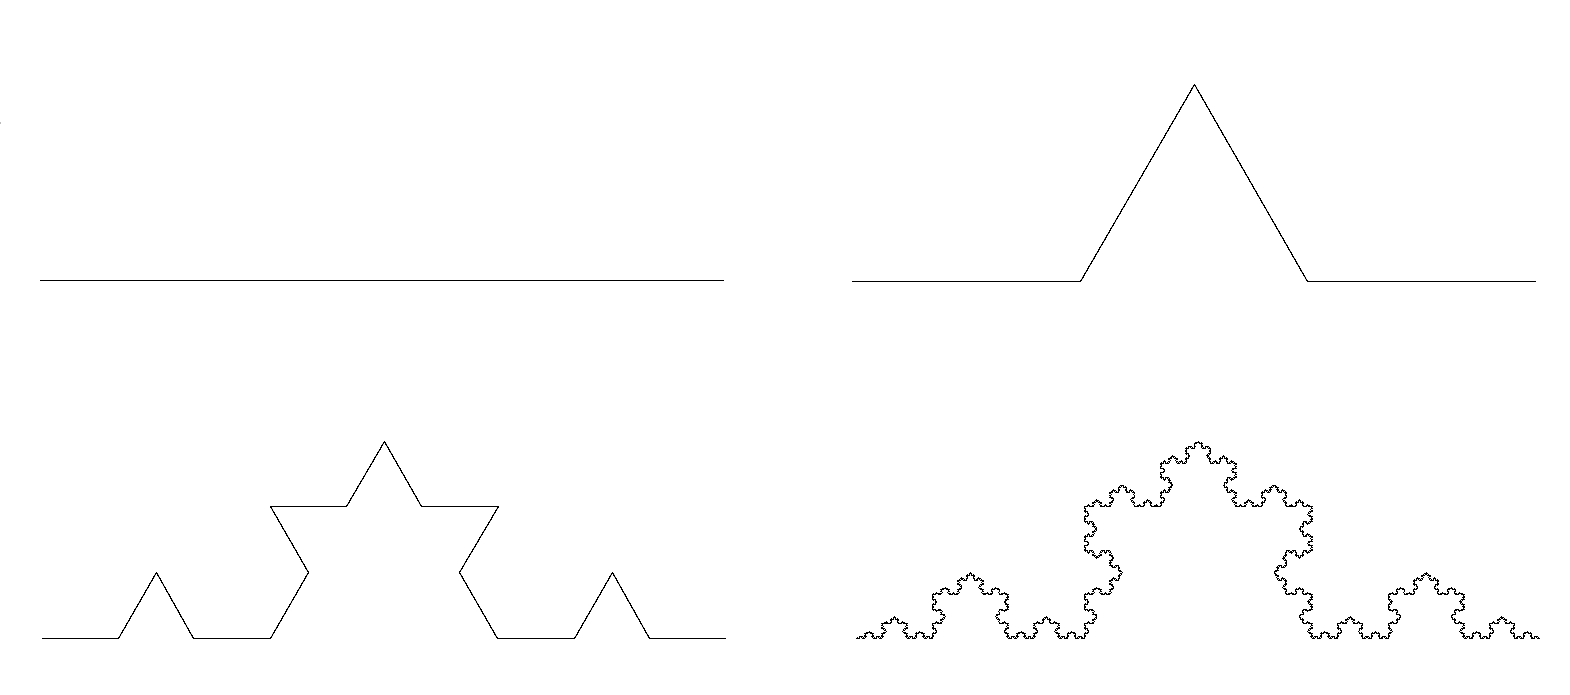
\includegraphics[width=.5\textwidth]{Pictures/Kochkurve.png}
    \caption{Die Entstehung der Kochkurve}
    \label{fig:Kochkurve}
\end{figure}
Wenn man in die Kochkurve hineinzoomt, findet man die Kochkurve immer wieder: ein rekursives Bild oder eben ein Fraktal (Prof. Dr. Guido Walz 2001, S. 128).\\Man definiert nun das Fraktal als eine Figur, bei der sehr oft Selbstähnlichkeit auffindbar ist, das heisst, dass das gesamte Fraktal oder Teile davon mehrfach im Fraktal vorkommen und das Fraktal selbst eine gebrochene und somit keine ganzzahlige Dimension besitzt (Bertram Maurer 2015, S. 258).\\

\subsubsection{Mandelbrotmenge}
Die nach dem Mathematiker Benoît B. Mandelbrot (*20.11.1924; †14.10.2010) benannte Menge ($\mathbb{M}$) beinhaltet jede Zahl $c$, die nicht gegen $\infty$ divergiert für die rekursive Folge (Reinhart Behr 1989, S. 54):
\begin{align*}
z_0&=0\\
z_{n+1}&=z^2_n+c
\end{align*}
Man fand heraus, dass wenn $|z_n| > 2$ gilt, wird die Folge gegen $\infty$ divergieren (Reinhart Behr 1989, S. 74).\\
Die erstellte Abbildung ergibt ein sehr schönes Gebilde, dem auch Farbe dazugegeben werden kann. Personen des deutschen Sprachraums sahen aufgrund seiner Form ein ’Apfelmännchen’ und nannten diese Abbildung danach (Reinhart Behr 1989, S. 54).\\
Die $\mathbb{M}$ ist ein Fraktal (Bertram Maurer 2015, S. 258). Man findet das erst gesehene Bild der Menge beim Hineinzoomen immer wieder. Somit ist es ebenfalls selbstähnlich. Immer wieder findet man im Mandelbrot verschiedene Julia-Mengen mit dem zugehörigen $c$ (Reinhart Behr 1989, S. 54). Diese sind ebenfalls Fraktale und selbstähnlich. $\mathbb{M}$ besitzt durch die vorgegebene Formel ein chaotisches System (Reinhart Behr 1989, S. 32).\\
All diese Faktoren führen sicherlich dazu, dass es einige YouTube-Videos gibt, die einen Zoom in die Menge zeigen, welche zur Herstellung auch viel Rechenleistung benötigen.
\begin{figure}[h]
	\centering
	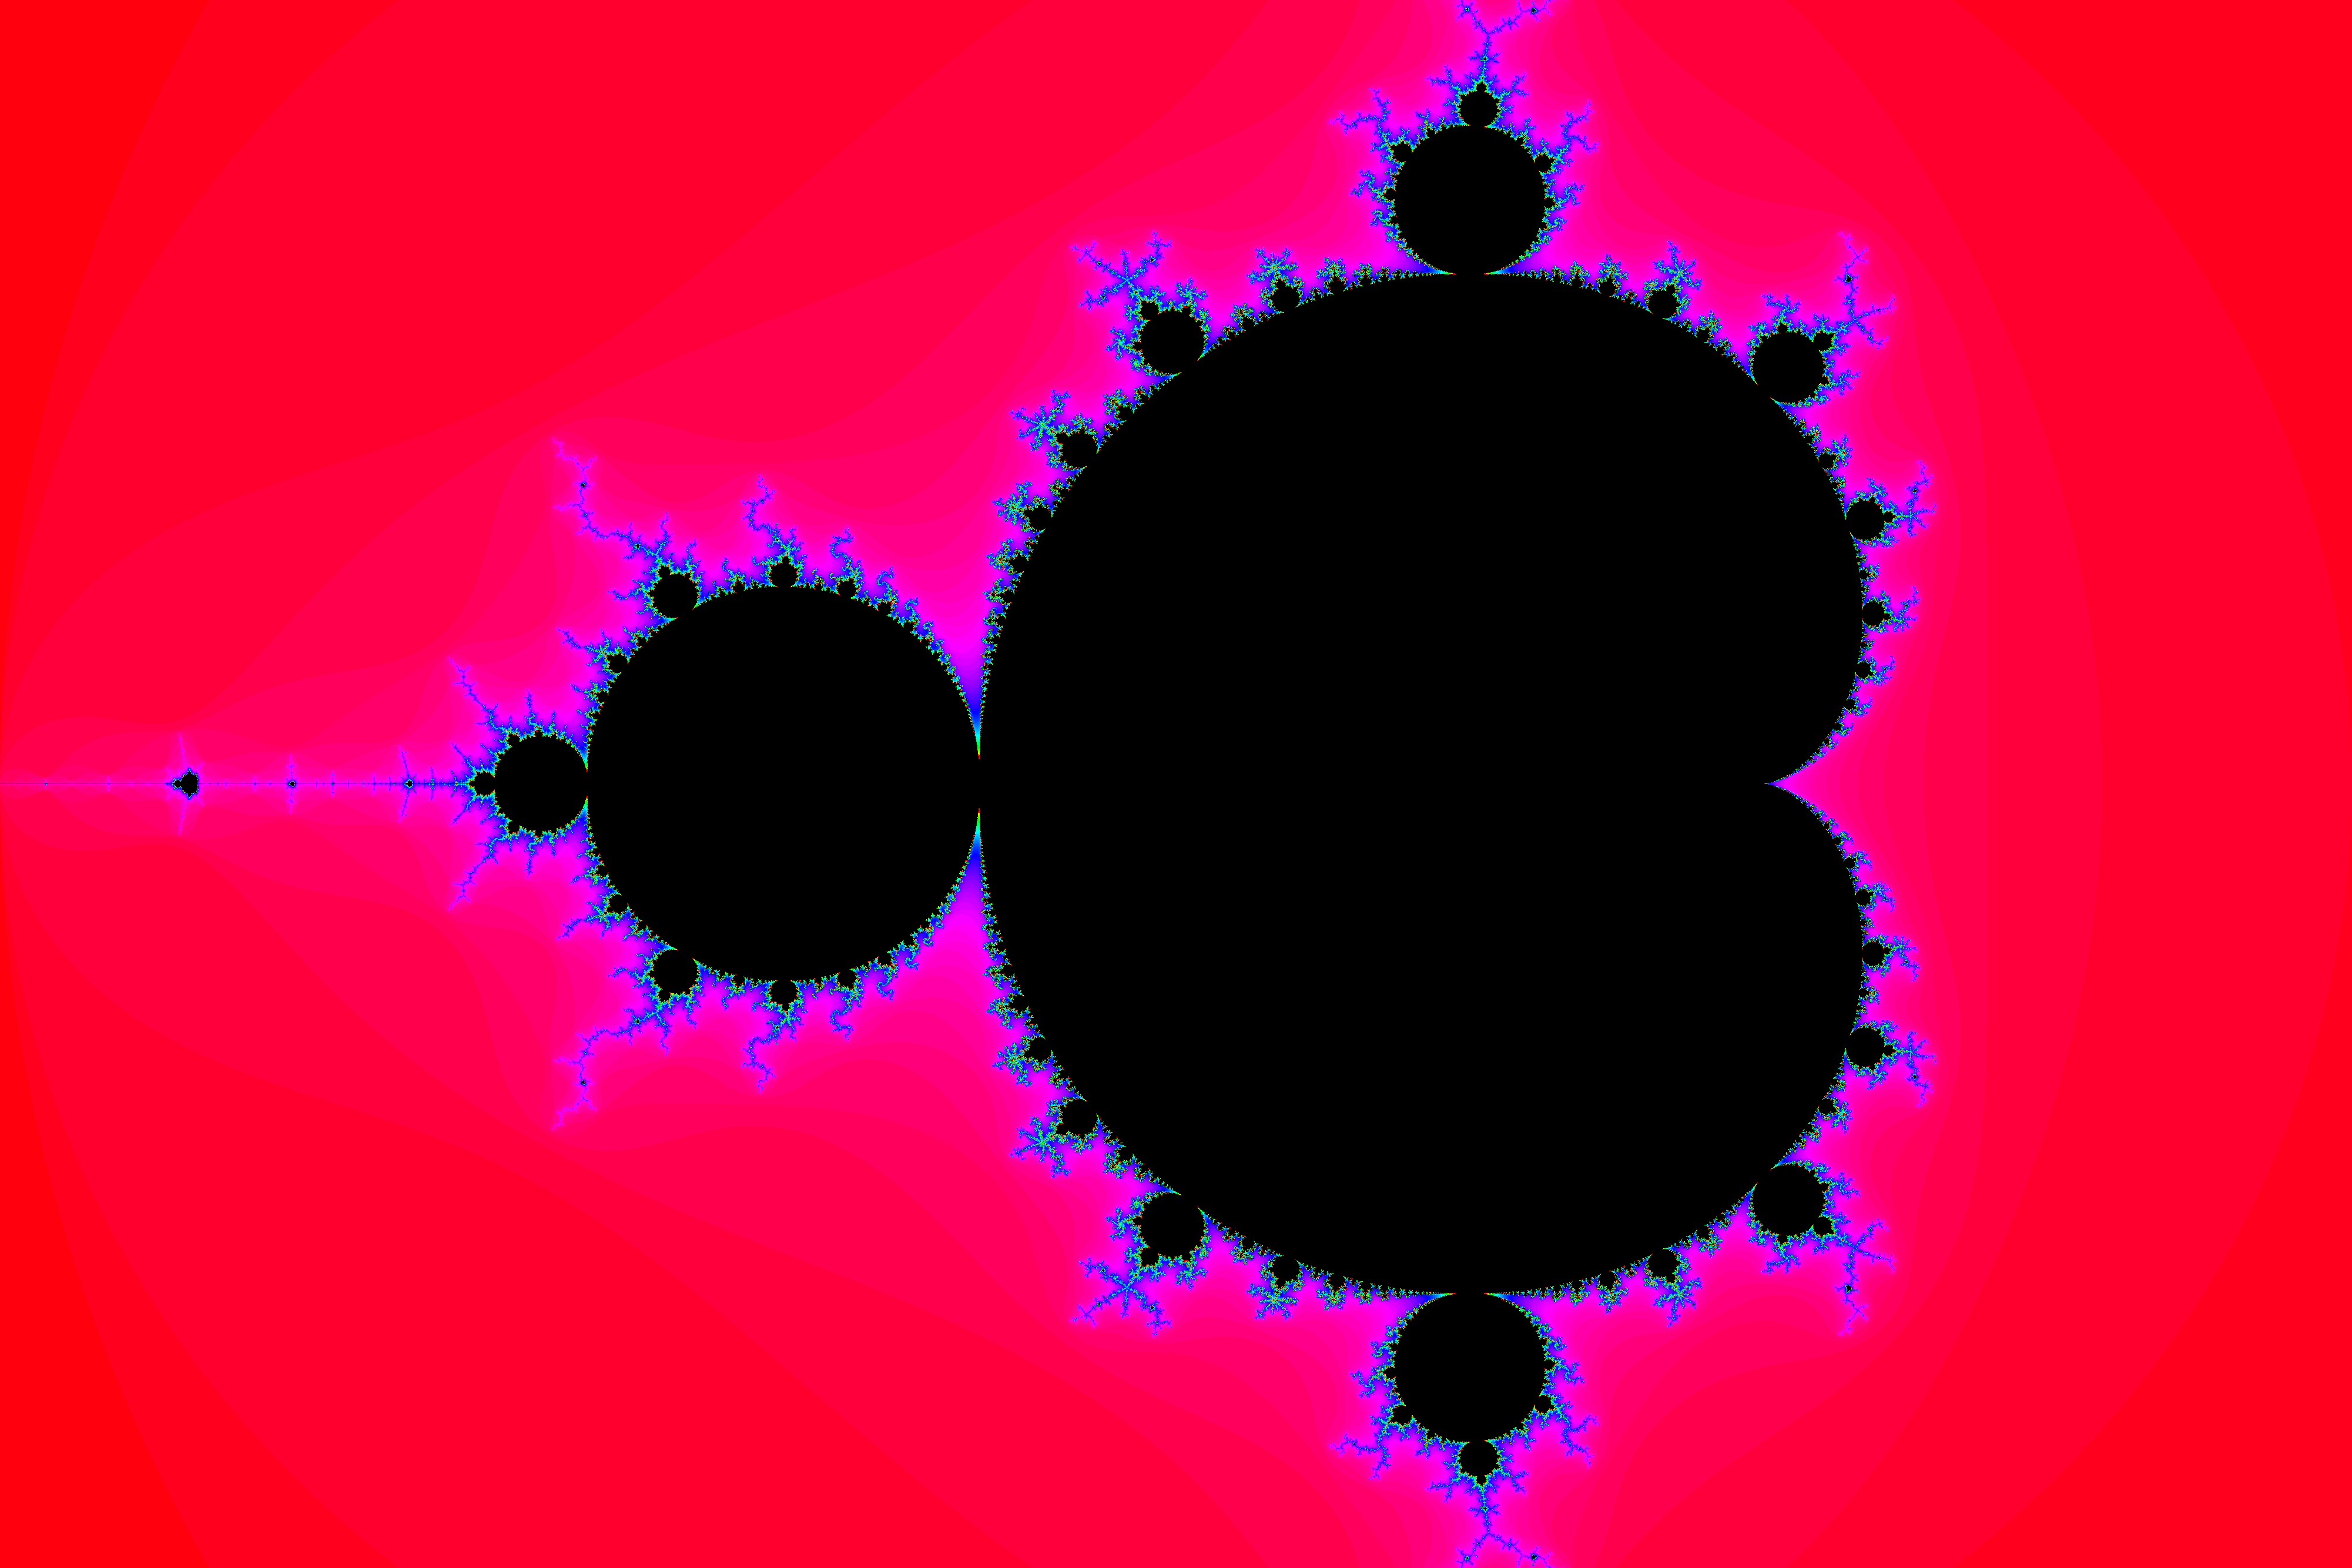
\includegraphics[width=.5\textwidth]{Pictures/Mandelbrot2668x4002.png}
	\caption{Das Mandelbrot, die $\mathbb{M}$ wird hier schwarz dargestellt}
	\label{fig:Mandelbrot}
\end{figure}
\newpage
\subsubsection{Buddhabrot}
Wenn man sich diese Abbildung als Erstes anschaut, ist der meditierende Buddha darin ersichtlich. Daher auch der Name ’Buddhabrot’. Das ‘Brot’ ist eine Andeutung, dass diese Abbildung etwas mit dem Mandelbrot zu tun hat, denn es stellt eine andere Variante dar, die $\mathbb{M}$ abzubilden.\\ 
Das Bild zum Buddhabrot entsteht, indem das Mandelbrot nochmals berechnet wird, allerdings nur die Punkte, die bei der Mandelbrotberechnung gegen das $\infty$ divergieren. Nun wird auch nicht mehr geschaut, nach wie vielen Schritten der Punkt $c$ ins $\infty$ abdriftet, sondern bei welchen Punkten $c$ nach jeder Iteration landet.\\
Zudem wird ein Zoom in das Buddhabrot durch das chaotische System von $\mathbb{M}$ und durch die fraktalen und selbstähnlichen Eigenschaften von $\mathbb{M}$ interessant (Melinda Green 2017).
\begin{figure}[h]
	\centering
	\includegraphics[width=.5\textwidth]{Pictures/BuddhabrotmengeWithZoomGPU1ToPoint-0.5 + 0.0imWithIteration1000withResolution9000x6000high.png}
	\caption{Das Buddhabrot}
	\label{fig:Buddhabrot}
\end{figure}